\documentclass{CRPITStyle}

\usepackage{harvard}
\usepackage{graphicx}

\pagestyle{empty}
\thispagestyle{empty}

\title{Lightweight Update Propagation using Atom}
\author{David W.\ Williamson \and Nigel J.\ Stanger}
\affiliation{Department of Information Science, \\
	University of Otago, \\
	PO Box 56, Dunedin, New Zealand \\
	Email:~\texttt{\{dwilliamson,nstanger\}@infoscience.otago.ac.nz}}


\begin{document}


\maketitle


\begin{abstract}
There are many situations where some form of automated update
propagation across disparate databases may be beneficial. For example, a
retailer could automatically retrieve the latest pricing data from their
suppliers' databases, and use these data to update their own internal
database. Doing so at regular intervals ensures that the retailer always
has current pricing information in their database. Electronic Data
Integration (EDI) tools that provide such features already exist but can
be expensive to implement, particularly for small to medium enterprises
(SME's). In this paper we propose a lightweight approach for propagating
updates from one database to another using the Atom XML syndication
format, thus providing a simpler, cost-effective technology for
facilitating data integration. This approach enables a target database
to regularly poll one or more source databases for updates, which are
then applied to the target database (alternatively, updates could be
``pushed'' to the target from the sources). This approach can be used in
typical data integration scenarios where the data sources are updated at
irregular intervals, such as the aforementioned retailer example, or
when extracting data from multiple data sources for loading into a data
warehouse. In the paper we discuss the underlying principles and
motivation for the approach, discuss possible architectures, and
describe an early prototype implementation.
\end{abstract}
\vspace{.1in}

\noindent {\em Keywords:} update propagation, data integration, Atom,
SME, lightweight architecture, Semantic Web, B2B


\section{Introduction}
\label{sec-intro}

The ability to integrate data from multiple heterogeneous sources is
becoming a key issue for modern businesses, and yet the number of
businesses implementing data integration solutions is smaller than we
might expect \cite{Beck-R-2002-Bled,vaHe-E-1999-EDI}. This is
particularly true for small to medium enterprises (SME's), for whom the
cost of implementing an enterprise-scale data integration solution can
often be prohibitive
\cite{Beck-R-2002-Bled,Guo-J-2003-DocEng,Somm-RA-2002-SIGMOD}.

In this paper, we propose a lightweight architecture for propagating
updates from one database to another using the Atom XML syndication
format. This architecture could provide a cost-effective alternative
technology for SME's to facilitate data integration rather than having
to purchase expensive enterprise grade systems. It is flexible and can
be easily extended to support additional functionality. We have
implemented a basic proof of concept of this architecture, and are
currently evaluating it using three case studies.

We should clarify at this point that we are not proposing an
architecture for processing data streams \cite{Babc-B-2002-Streams}.
Such architectures deal with processing continuous streams of real-time
data, whereas our architecture provides a lightweight means to propagate
discrete sets of ``conventional'' update operations from one database to
another.

The body of this paper comprises four main sections. In
Section~\ref{sec-background} we provide some general background
information regarding data integration and the Atom syndication format.
In Section~\ref{sec-motivation} we discuss the motivation behind our
proposed architecture. We then discuss the proposed architecture and the
goals of our research in Section~\ref{sec-architecture}, and present
some possible directions for future work in
Section~\ref{sec-future-work}. The paper concludes in
Section~\ref{sec-conclusion}.


\section{Background}
\label{sec-background}

In this section, we briefly discuss the concepts and technologies that
underlie our proposed architecture. In
Section~\ref{sec-data-integration} we provide a brief overview of data
integration, especially in the context of SME's attempting to implement
a data integration solution. This is followed by a brief discussion of
the development of Atom and related technologies such as RSS and RDF.


\subsection{Data Integration}
\label{sec-data-integration}

Data integration is a term used to describe the combining of data
residing in different sources to provide the user with a unified view of
data \cite{Bati-C-1986,Yu-C-2004-SIGMOD}. This activity is becoming
increasingly important to modern business operation as more and more
organizations rely upon applications that support staff in undertaking
informed decision making \cite{Calv-D-1998-CoopIS,Yu-C-2004-SIGMOD}.

Data integration is a domain that has been a topic of research for some
time \cite{Beck-R-2002-Bled,Wied-G-1993-SIGMOD}; today this domain is of
no less significance with many organizations requiring the aggregation
of data from multiple and often heterogeneous sources, for a wide
variety of applications \cite{Haas-LM-1999-DEB}.
\citeasnoun{Bati-C-1986} illustrated three common scenarios for
integration environments:

\begin{itemize}

	\item homogeneous, where all the sources of data share the same
	schema;

	\item heterogeneous, where data must be integrated from sources that
	may use different schemas or platforms (e.g., a combination of
	relational and hierarchical databases); and

	\item federated, where integration is facilitated by the use of a
	common export schema over all data sources.

\end{itemize}

A typical example of data integration from heterogeneous sources can be
found in the arena of business-to-business (B2B) commerce, where, for
example, a manufacturer may have to interact with multiple suppliers or
temporary contractors, each of whom may use completely different data
structures and data exchange formats \cite{Ston-M-2001-SIGMOD}. With the
introduction of cheaper web based technology, many additional
organizations have been able to undertake projects to facilitate data
integration, but the costs associated with such technology can still be
quite prohibitive to the many smaller companies and organizations that
comprise the majority of most countries' economies.

Many initiatives have been put forward to try and alleviate this
situation, one of the more recent being the OASIS Universal Business
Language (UBL) standard \cite{Mead-B-2004-UBL}, which is a project to
standardize common business documentation---invoices, purchase orders,
etc.---so that it is easier for companies to establish and maintain
automated transactions with other parties. UBL has been designed to
operate with ebXML.

XML has been widely adopted as a standard platform for exchanging data
between organizations, and many specialist standards---such as the
aforementioned ebXML---have been developed to cater to the unique needs
that certain business sectors present. In addition to XML-based language
specifications, other standards such as EDIFACT and EXPRESS have been
defined to facilitate the transmission of information from various
sources so that it may be integrated with other data.


\subsection{The Atom Syndication Format}
\label{sec-atom-overview}

In this section we provide a brief overview of the Atom syndication
format and the technologies that led to its development.


\subsubsection{RDF, RSS and the Semantic Web}
\label{sec-rdf-rss}

The World Wide Web (WWW) as it stands today mostly comprises documents
intended for humans to read, i.e., ``\ldots{}a medium of documents for
people rather than for data and information that can be processed
automatically\ldots'' \cite{Bern-T-2001-SciAm}, which provides minimal
opportunity for computers to perform additional interpretation or
processing on them \cite{Bern-T-1999-WWW,Bern-T-2001-SciAm}. In essence,
computers in use on the Web today are primarily concerned with the
parsing of elementary layout information, for example headers, graphics
or text, and processing like user input forms
\cite{Bern-T-1999-W3C,Bern-T-2001-SciAm}.

There are few means by which computers can perform more powerful
processing or manipulation on web resources
\cite{Bern-T-2001-SciAm,Fens-D-2003}, most often because the additional
semantics required do not exist or are not in a form that can be
interpreted by computers \cite{Koiv-MR-2001-W3C}. The motivation for the
adoption of semantics in Web documents can be made evident simply by
using a contemporary search engine to look for an ``address''. This
search may well return a plethora of results ranging from street
addresses and email addresses to public addresses made by important
individuals through the ages.

This kind of scenario is one of the reasons for the W3C's Semantic Web
project \cite{Koiv-MR-2001-W3C}. In the words of its creator, Tim
Berners-Lee, its goal is to:

\begin{quotation}
	``\ldots{}develop enabling standards and technologies designed to help
	machines understand more information on the Web so that they can
	support richer discovery, data integration, navigation, and
	automation of tasks. With Semantic Web we not only receive more
	exact results when searching for information, but also know when we
	can integrate information from different sources, know what
	information to compare, and can provide all kinds of automated
	services in different domains from future home and digital libraries
	to electronic business and health services.'' \cite{Koiv-MR-2001-W3C}
\end{quotation}

In other words, the Semantic Web will provide a space where more
intelligent searching and processing of information will be made
possible by further extending the existing capabilities of the World
Wide Web (WWW).

RDF is a technology that is an integral part of the W3C Semantic Web
initiative, as the following excerpt from the W3C Semantic Web activity
statement will attest:

\begin{quotation}
	``The Resource Description Framework (RDF) is a language designed to
	support the Semantic Web, in much the same way that HTML is the
	language that helped initiate the original Web. RDF is a framework
	for supporting resource description, or metadata (data about data),
	for the Web. RDF provides common structure that can be used for
	interoperable XML data exchange.'' \cite{Powe-S-2003-RDF}
\end{quotation}

What RDF does in the context of the Semantic Web is to provide a way to
record data so that they can be interpreted easily by machines, which in
turn provides an avenue to ``\ldots{}more efficient and sophisticated
data interchange, searching, cataloguing, navigation, classification and
so on\ldots{}'' \cite{Powe-S-2003-RDF}.

Since its inception in the late 1990's, the RDF specification has
spawned several applications, RSS being but one example. RDF Site
Summary (RSS) is an XML application, of which versions 0.9 and 1.0
conform to the W3C's RDF specification. It is a format intended for
metadata description and content syndication \cite{Mano-F-2004-RDF}.
Originally developed by Netscape as a means to syndicate content from
multiple sources onto one page \cite{Nott-M-2005-Atom}, RSS has been
embraced by other individuals and organizations resulting in the
spawning of multiple versions.

At its most simple, the information provided in an RSS document
comprises the description of a ``channel'' (which could be on a specific
topic such as current events, sport or the weather, etc.) consisting of
URL linked items. Each item comprises a title, a link to the actual
content and a brief description or abstract.

Because of the proliferation of differing RSS standards and associated
problems with compatibility, a group of service providers, vendors and
developers have initiated the development of a separate syndication
standard named Atom, which will, according to the Atom Publishing Format
and Protocol (Atompub) Working Group, be heavily influenced by the
lessons learned in the evolution of RSS.


\subsubsection{Atom}
\label{sec-atom-detail}

The Atom specification defines an XML-based document format that is
designed to describe lists of related information
\cite{Nott-M-2005-Atom}. These lists are known as ``feeds''. Feeds are
made up of multiple items, known as ``entries''; each entry can have an
extensible set of attached metadata \cite{Nott-M-2005-Atom}.

Atom as a technology comprises four key related components: a conceptual
model of a resource, a well defined syntax for this model, the actual
atom feed format itself and the editing protocol. Both the feed format
and editing protocol also make use of the aforementioned syntax.

In addition to these features, the Atompub Working Group have outlined
several design objectives for the feed format and the editing protocol.
The feed format must be able to represent the following: a resource that
is a weblog entry or article, a feed or channel of entries, a complete
archive of all entries within a feed, existing well formed XML
content (especially XHTML), and additional information in a
user-extensible manner.

The editing protocol must support creating, deleting or editing feed
entries, multiple authors for a single feed, user authentication, user
management, and the ability to create, obtain and configure
complementary material such as comments or templates.

The latest specification of Atom, which at the time of writing is still
in draft form, states that the main purpose that Atom is intended to
address is ``\ldots{}the syndication of Web content such as Weblogs and
news headlines to Web sites as well as directly to user agents''
\cite{Nott-M-2005-Atom}. The specification also suggests, however, that
Atom should not be limited to just web based content syndication but in
fact could be adapted for other uses or content types. The Atompub
Working Group aim to submit the Atom feed format and editing protocol to
the IETF for consideration as a proposed standard in early April 2005.


\section{Motivation}
\label{sec-motivation}

One of the example domains of data integration is that of Electronic
Data Interchange (EDI), a concept used by companies to exchange
information such as goods procurement documentation. EDI is not new
\cite{Beck-R-2002-Bled,Medj-B-2003-VLDB}, and has been used for many
years by various organizations to reduce costs by replacing more
traditional paper based systems. It is interesting to note, however,
that in surveys regarding the extent of adoption of EDI, only a fraction
of the companies that might be perceived as beneficiaries of such
technology have actually implemented or attempted to implement it
\cite{Beck-R-2002-Bled,vaHe-E-1999-EDI}. This naturally raises the
question of why this is the case. We can further refine this question by
asking why so few smaller companies (SME's) have adopted EDI or indeed
other technologies that rely on accurate automated data integration,
such as data warehousing.

Perhaps the most important reason is that of cost: to a small company
the perceived benefits of introducing the technology may not be
sufficient to justify the expense
\cite{Beck-R-2002-Bled,Guo-J-2003-DocEng,Somm-RA-2002-SIGMOD}. When a
decision has been made to implement new technology, it is often the case
that the SME in question has been forced into an investment that is, to
them, an expensive solution, perhaps due to demands imposed by larger
clients and partners, or as a response to competitors in an attempt to
maintain market position \cite{Beck-R-2002-Bled,vaHe-E-1999-EDI}.

Attempts have been made to make EDI more cost effective by introducing
EDI on a web-based platform \cite{Beck-R-2002-Bled}, and through the
development of standards such as the recently sanctioned OASIS Universal
Business Language (UBL) standard \cite{Mead-B-2004-UBL}. While UBL is
new and has probably not had sufficient time to make a substantial
impact, the fact remains that the underlying reason these types of
technologies are still not attractive enough to SME's is cost
\cite{Beck-R-2002-Bled,Guo-J-2003-DocEng,Somm-RA-2002-SIGMOD,vaHe-E-1999-EDI}.

To summarize, data integration related technologies are often not
readily or willingly implemented by SME's because of the perceived high
costs involved, and at best are implemented only if it is deemed vitally
important to the continued survival of the organization in the
marketplace.

Such a situation leads us to the conclusion that there is a need for
alternative data integration technologies that are cost effective,
enabling SME's to embrace the benefits of applications that use data
integration technologies, such as data warehousing, EDI networks or
e-catalogues.

This identified need provides the motivation for our proposed
architecture, which we will discuss in the next section.


\section{Proposed Architecture, Implementation and Methodology}
\label{sec-architecture}

To facilitate the adoption of data integration in SME's, we propose a
lightweight architecture for propagating database updates based on Atom,
as illustrated in Figure~\ref{fig-basic}. Atom was chosen as the
underlying technology because of its XML heritage, and because the Atom
community is trying to encourage different uses for the format beyond
the traditional application of weblog syndication
\cite{Nott-M-2005-Atom}. Although the standard has yet to be officially
ratified, it already has a large user and development community.
%%!! check ratification status

\begin{figure*}[htb]
	\fbox{\parbox[b]{.99\linewidth}{%
		\vskip 0.5cm%
		\centerline{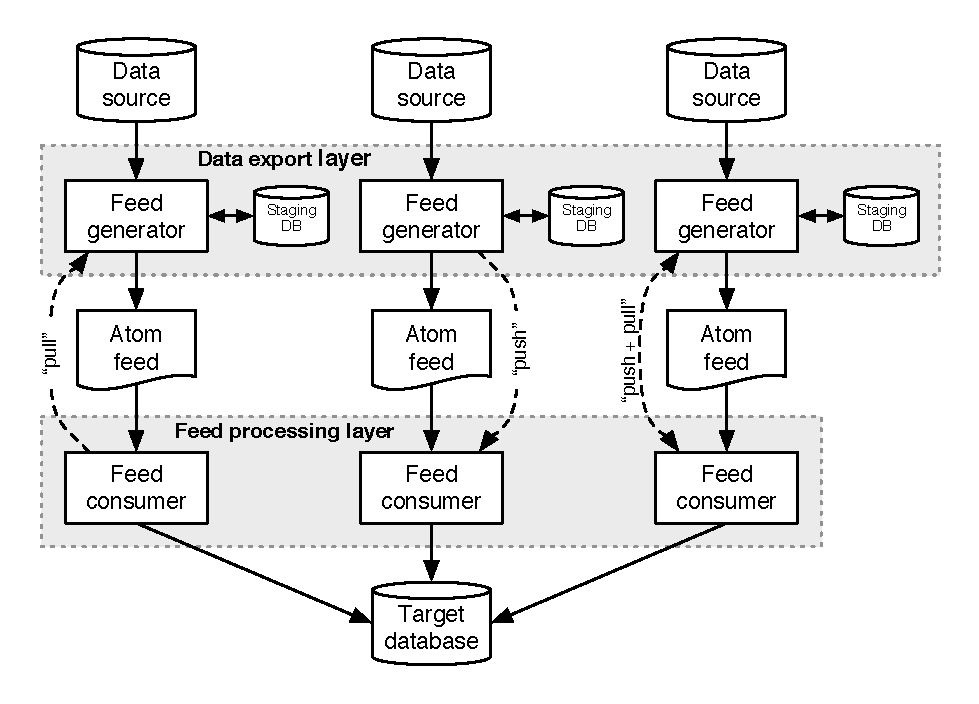
\includegraphics[scale=0.9]{Architecture_basic}}%
		\vskip 0.5cm%
	}}
	\caption{Overview of the basic architecture}
	\label{fig-basic}
\end{figure*}

The ``feed consumer'' modules shown in Figure~\ref{fig-basic} take as
input Atom feeds from client sources, which simulate incoming data from
client or supplier data sets. Two different methods of implementation
have been explored, categorised as ``push'' and ``pull''---the names
referring to how the flow of feed data to the target schema is managed.

Within the push method, the consumption of feed information is governed
predominantly by changes in state of the source data, i.e., when the feed
generator detects a change in state of the source data (for example when
a record is updated) the feed is regenerated and the consumer module
called immediately to apply the new information to the target schema. 
The majority of this activity takes place at or near the source data location,
however in practice the location of each component is not too critical as
they are web-based.

The pull method however differs from the push approach on two
key points. First, the feed consumer modules operate independently of,
and are therefore not directly influenced by, the feed generator
component and second, the flow of feed information to the target schema
is governed by the consumer module itself, i.e., the consumer module
will regularly check or ``poll'' the Atom feed to see if it has changed
or not since the last time (this is done by simply checking the Atom
feeds <modified/> content). Hence rather than forcing or pushing feed
data, it is instead pulled down to the target.

A further improvement to this design has been proposed, whereby the
consumer module polls the feed generator directly at which point if the
feed generator has changed since last time it generated a feed and
informs the consumer module of the feed's location. It is thought that
this method would reduce the possibility of updates being lost and allow
feeds to be dynamically created on demand rather than the static
feed generation approach used in the current prototype implementation.

In order to evaluate the prototype, we have implemented two different
simulated scenarios derived from actual use case of previous projects.
Both case studies follow a similar structure whereby data will be
exported as Atom feeds from the source database(s), which are then read 
by the consumer module before being sent to the target.

The first scenario simulates the integration of movie timetable data
from multiple cinema databases into a vendors' movie timetable database.
This database is used to populate an e-catalogue allowing users to query
times and locations for movies currently screening at cinemas
contributing data to the system. The Atom feeds in this scenario
represent flows of data from the supplier (the participating cinemas) to 
the vendor (the e-catalogue provider).

The second scenario follows on from an earlier research project undertaken
at Otago University to develop a kiosk-based system for the sale and 
distribution of music in digital format, e.g., MP3.

The database a kiosk uses is populated with information from vendors who
have agreed to supply content, i.e., music files. In this case, the
prototype acts as a mechanism to propagate data and changes to existing
data in the suppliers' data sources to the music kiosk system's own
database---the target. The Atom feeds in this instance are used to
maintain an up to date database that has the location and description of
each available music track for sale in the system.

Both case studies had a varying level of complexity in terms of design
and implementation demands, which allowed us to pursue a staged
development of the core components by starting with the less complicated
of the case studies first, the movie e-catalogue, and then building on 
what was learned and extending what we had created in order to complete 
the music kiosk system implementation.

Essential functionality testing on the movie e-catalogue system will be
carried out, however, more intensive testing is being focused on the 
music kiosk retail system because it not only contains all the same 
features as found in the first but also reflects more aspects of 
functionality that would be found in many other real world projects, with
its added feature to update existing records held within the target schema.
In addition, the volume of data involved was much greater than that in the
movie e-catalogue system which meant that the music kiosk system provided
an excellent opportunity to test an Atom based system under a variety of 
loading conditions.

The testing environment currently consists of five Apple PowerMac G5
computers with dual 1.8 GHz CPU's and 1 GB of RAM. The computers are 
connected via a full duplex gigabit eithernet network using a Dell PowerConnect
2624 series switch. Software required for the system consists of a Web server,
PHP, database server and a Web browser, for which we have used Apache 1.3.33, 
PHP 5.0, MySQL4.? and Firefox 1.0.6 respectively. Four of the Apple computers 
are used as data sources with each having a source schema installed while the 
fifth computer is used to house the target schema. 

A set of sample data was generated that ranged in equivalent size of 5600 to
22400 rows. For each set of sample data, four ``runs'' are made with each run having
an additional data source added i.e. the first test run has one data source, the
second has two and so on. This approach allows us to view not only how the 
system performs when dealing with increasingly larger amounts of data but also
with varying numbers of ``physical'' data sources.

Preliminary load testing to date has yielded data for the push method
prototype pertaining to the time taken to propagate a set of records.
The size of sample data used in testing ranged between 5600 to over 
80,000 rows. In addition, the size of the generated Atom feed and the 
SQL generated for the target schema was also recorded.


%We are currently implementing a basic proof of concept of this
%architecture, and will evaluate its cost-effectiveness and performance
%compared to other data integration technologies. The prototype builds
%upon existing software available for processing Atom feeds, and adds a
%module (written in PHP) for integrating incoming data from different
%feeds.
%
%The integration module takes as input Atom feeds from multiple data
%sources, which simulate incoming data from client or supplier data sets.
%(For the initial prototype we have assumed that the data feeds are
%homogeneous; obviously this will need to be extended to heterogeneous
%feeds in later versions.) After the Atom feeds have been collected, the
%integration module will integrate the data supplied by the feeds into a
%schema that matches that of the target database, as shown in Figure 1. A
%transaction simulator will be employed to simulate workload and updates
%to the source databases, in order to recreate a day-to-day production
%environment.
%
%In order to evaluate the prototype, we will implement three different
%simulated scenarios derived from actual use cases of previous projects.
%All three case studies follow a similar structure whereby data will be
%exported as Atom feeds from the source database(s), which are then
%consumed by the integration module before being sent to the target
%database for insertion.
%
%The first scenario will simulate the integration of product data from
%multiple suppliers into a vendor's product information database. The
%product information database is used to populate the vendor's online
%product catalogue, which clients use to make decisions regarding goods
%procurement. The Atom feeds in this scenario represent flows of product
%data from the supplier to the vendor.
%
%The second scenario follows on from an earlier research project to
%develop a kiosk system for the sale and distribution of music in digital
%format. The database the kiosk(s) use will be populated with information
%from vendors who have agreed to supply content (e.g., a record label's
%collection of music files). What is needed is a mechanism to integrate
%all the music data from each supplier into the music kiosk system's own
%database. The Atom feeds in this scenario are used to maintain an up to
%date database that has the location and description of each available
%music track for sale in the system.
%
%The third scenario will simulate the implementation of a data
%warehousing solution for a computer components distributor.
%
%Preliminary results from the case study evaluations are expected to be
%available by June 2005. Our primary goal with the initial prototype is
%to prove the feasibility of our approach. We will compare our proposed
%architecture against existing data integration solutions by means of a
%cost/benefit analysis. We may also investigate measuring various
%software quality characteristics as defined by the ISO 9126 standard
%\cite{ISO-2001-9126-1}.


\section{Future Work}
\label{sec-future-work}

As the initial prototype is intended as a basic proof of concept of the
proposed architecture, it has been kept as simple as possible in order
to facilitate implementation and evaluation. There are several obvious
extensions to the basic prototype that will be investigated in later
iterations of the architecture.

The initial prototype assumes that all data sources are largely
homogeneous, that is, that they all share similar semantics and can
therefore be relatively easily integrated. An obvious extension is to
permit heterogeneous data sources that have differing semantics. This
would require the addition of export and mapping schemas, and a schema
mapping layer to map incoming data from the source schema to the target
schema, as shown in Figure~\ref{fig-extended}. These components could
perhaps make use of the W3C's Web Ontology Language (OWL)
\cite{McGu-DL-2004-OWL}.

\begin{figure*}[htb]
	\fbox{\parbox[b]{.99\linewidth}{%
		\vskip 0.5cm%
		\centerline{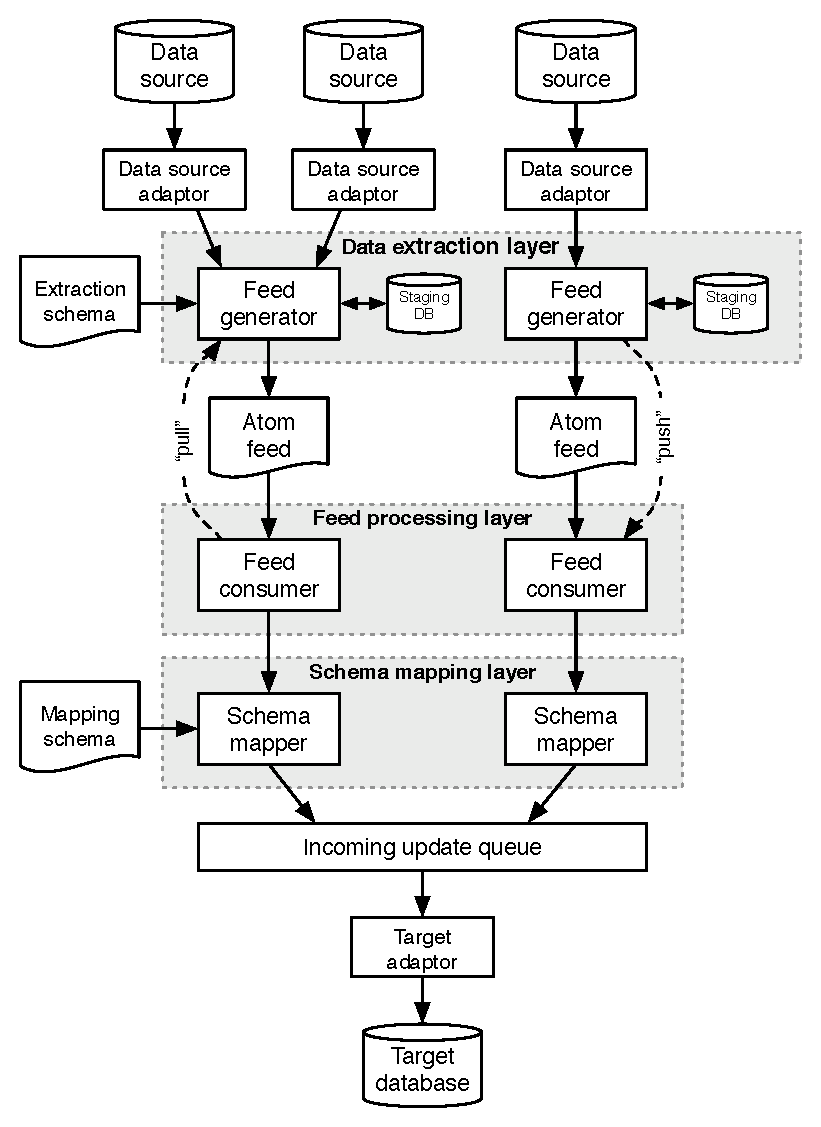
\includegraphics[scale=0.9]{Architecture_extended}}%
		\vskip 0.5cm%
	}}
	\caption{Possible extensions to the architecture}
	\label{fig-extended}
\end{figure*}

The prototype also assumes only a single ``author'' per Atom feed, that
is, there is only a single database underlying each feed (as implied by
Figure~\ref{fig-basic}). It is quite feasible to have a single data
source that is actually a view layered on top of a collection of
underlying databases, as illustrated at top left in
Figure~\ref{fig-extended} (e.g., a supplier might draw data for their
Atom feed from multiple databases within their organization). It would
therefore be useful to investigate the possibility of multiple
``authors'' per Atom feed.

The prototype currently only supports the PostgreSQL and MySQL database
management systems. While there has been some simple generalisation to
enable the system to work with with both products, an obvious extension
is to further generalise the data source interface to support multiple
relational and non-relational data sources and targets. This is
illustrated by the ``adaptor'' components in Figure~\ref{fig-extended}.

Another possible extension could be to generalise the ``transport
layer'' of the architecture. The architecture is currently based on Atom
feeds over HTTP, but could conceivably be generalised to support
different transport formats and protocols, such as Jabber, email, and so
on.

The data flows shown in Figures~\ref{fig-basic} and~\ref{fig-extended}
imply that the proposed architecture is one-way only (i.e., from the
data sources to the target database), but this may not be true in
general. It would therefore be interesting to investigate extending the
architecture to allow for the possibility of two-way data transfers,
i.e., allowing data to flow from the target back to the sources.


\section{Conclusion}
\label{sec-conclusion}

In this paper, we discussed a lightweight update propagation
architecture based on the Atom XML syndication format. Cost is a major
factor in the slow adoption of data integration technologies by small to
medium enterprises, so the proposed architecture could provide a
cost-effective alternative for implementing data integration
infrastructures in small business environments. We have developed a
basic proof-of-concept prototype system that will be evaluated using a
series of realistic case studies. We expect to have preliminary results
from these evaluations by June 2005.


\section*{Acknowledgements}
\label{sec-acknowledgements}

The authors would like to thank Dr. Colin Aldridge and Dr. Stephen
Cranefield for their helpful comments on an early draft of this paper.


\bibliographystyle{agsm}
\bibliography{Atom_updates}


\end{document}
